\documentclass[11pt]{report}
\renewcommand{\baselinestretch}{1.5}


% Declaração dos pacotes
\usepackage[utf8]{inputenc}
\usepackage[T1]{fontenc}
\usepackage{graphicx}
\usepackage[portuguese]{babel}
\usepackage{graphicx}
\usepackage[affil-it]{authblk} % Usado para meter nome da escola
\usepackage{eurosym} % Usado para o €
\usepackage{url} % URL



% CAPA
\title{\textbf{\textit{Desenvolvimento de uma estação meteorológica em bare-metal e RTOS. }\\
		\large1º Trabalho prático de
		Sistemas Embebidos e de Tempo Real }}
			
				
\author{Rúben Guimarães nº11156\\ Kyrylo Yavorenko nº10355 }

\affil{Escola Superior de Tecnologia, IPCA \\
	Barcelos}	
	
		
\date{06 de Maio de 2018}


\begin{document}

\maketitle




% Indice
\tableofcontents


% Introdução
\chapter*{Introdução}
\addcontentsline{toc}{chapter}{Introdução}


O trabalho prático abordado neste relatório foi desenvolvido no âmbito da unidade curricular Sistemas Embebidos e de Tempo Real do curso de Engenharia de Sistemas Informáticos, lecionada pelo docente António Moreira.\newline O docente desafiou os alunos a aplicarem os conceitos de programação de sistemas embebidos e de tempo real lecionados durante o decorrer da unidade curricular, surgindo assim este projeto, dividido em duas partes, (baremetal e usando o sistema operativo FreeRTOS), que adquire de diversas fontes de sinais analógicos e digitais informação replicando o funcionamento de uma estação meteorológica.


\clearpage



% Resumo
\chapter*{Resumo}
\addcontentsline{toc}{chapter}{Resumo}

Neste trabalho desenvolvemos uma pequena estação meteorológica recorrendo à plataforma de prototipagem eletrónica open-source Arduino. Esta estação consiste num conjunto de sensores que obtém dados sobre o estado do tempo que depois são enviados para o Arduino para serem processados, sendo por fim mostrados ao utilizador, quer através de um lcd de 16x2, quer através da consola do IDE do Arduino.


\clearpage


% Objectivos
\chapter*{Objetivos}
\addcontentsline{toc}{chapter}{Objetivos}

Os objetivos definidos para o projeto pelo docente foram:

\begin{itemize}
\item Desenvolvimento de um programa usando a tipologia baremetal.
\item Desenvolvimento de um programa usando o sistema operativo FreeRTOS usando 3 tasks.
\item Utilizar os seguintes sensores:
\begin{itemize}
\item Sensor de água.
\item 3 LDR's para calcular a posição do sol.
\item Sensor de humidade.
\item Dois sensores de temperatura (para o ar e o solo).
\item Barómetro.
\item Anemómetro 
\end{itemize}
\end{itemize}


\clearpage


% Arquitectura
\chapter*{Arquitetura}
\addcontentsline{toc}{chapter}{Arquitetura}

Podemos consultar na figura seguinte um diagrama com a arquitetura do projeto.


\begin{figure} [!h]
\centering
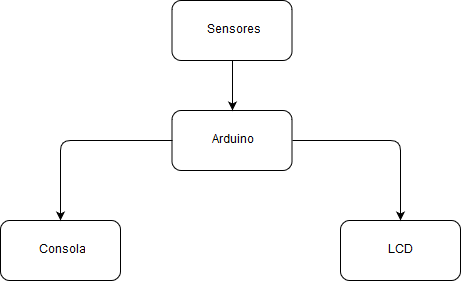
\includegraphics[width=\textwidth]{Prints/arquitectura.png}
\caption{Diagrama da arquitetura do projeto}
\label{Rotulo}
\end{figure}


\clearpage


% Recursos usados no projecto
\chapter*{Recursos usados no projeto}
\addcontentsline{toc}{chapter}{Recursos usados no projeto}

Para o desenvolvimento do projeto foram utilizados os seguintes recursos:

\textbf{Software:}
\begin{itemize}
\item \textit{Arduino IDE 18.5} para o desenvolvimento do código usado.
\item \textit{GitHub Desktop} para atualizar o repositório com o código do projeto.
\item \textit{Fritzing 0.9.3b} para criar os protótipos dos esquema do projeto.
\item \LaTeX \hspace{1mm} para a escrita do relatório.

\end{itemize}

\textbf{Hardware:}
\begin{itemize}
\item \textit{Arduino Mega 2560,} placa que contem o micro-controlador que controla todo o nosso projeto.
\item \textit{DHT11,} sensor usado para obter leituras de humidade e temperatura do ambiente.
\item \textit{DS18B20,} sensor à prova de água usado para obter temperaturas de água.
\item \textit{BMP180,} sensor que obtém leituras da pressão atmosférica e da temperatura ambiente. Com os valores obtidos conseguimos fazer uma estimativa da altitude.
\item \textit{Water Sensor,} sensor usado para saber se existe água ou não.
\item \textit{Buzzer,} usado para dar um feedback sonoro caso seja detetada água no sensor de água.
\item \textit{QTR-8RC,} sensor usado para contar as rotações por minuto de um cata-vento.
\item \textit{LCD 16x2,} usado para mostrar os valores obtidos pelos sensores.
\item \textit{Light Dependent Resistor,} usado para descobrir qual das posições (sul, este ou oeste) o sol de encontra.
\item \textit{Breadboard,} usada para montar o circuito.
\item \textit{Diversas resistências,} usadas para proteger componentes ou para servir de pull-up.
\item \textit{Diversos fios,} usados para efetuar as ligações entre os componentes, breadboard e o arduino.

\end{itemize}



% Esquema do projecto
\chapter*{Esquema do projeto}
\addcontentsline{toc}{chapter}{Esquema do projeto}

Na imagem seguinte podemos verificar o esquema do projeto desenvolvido na plataforma fritzing.

\begin{figure} [!h]
\centering
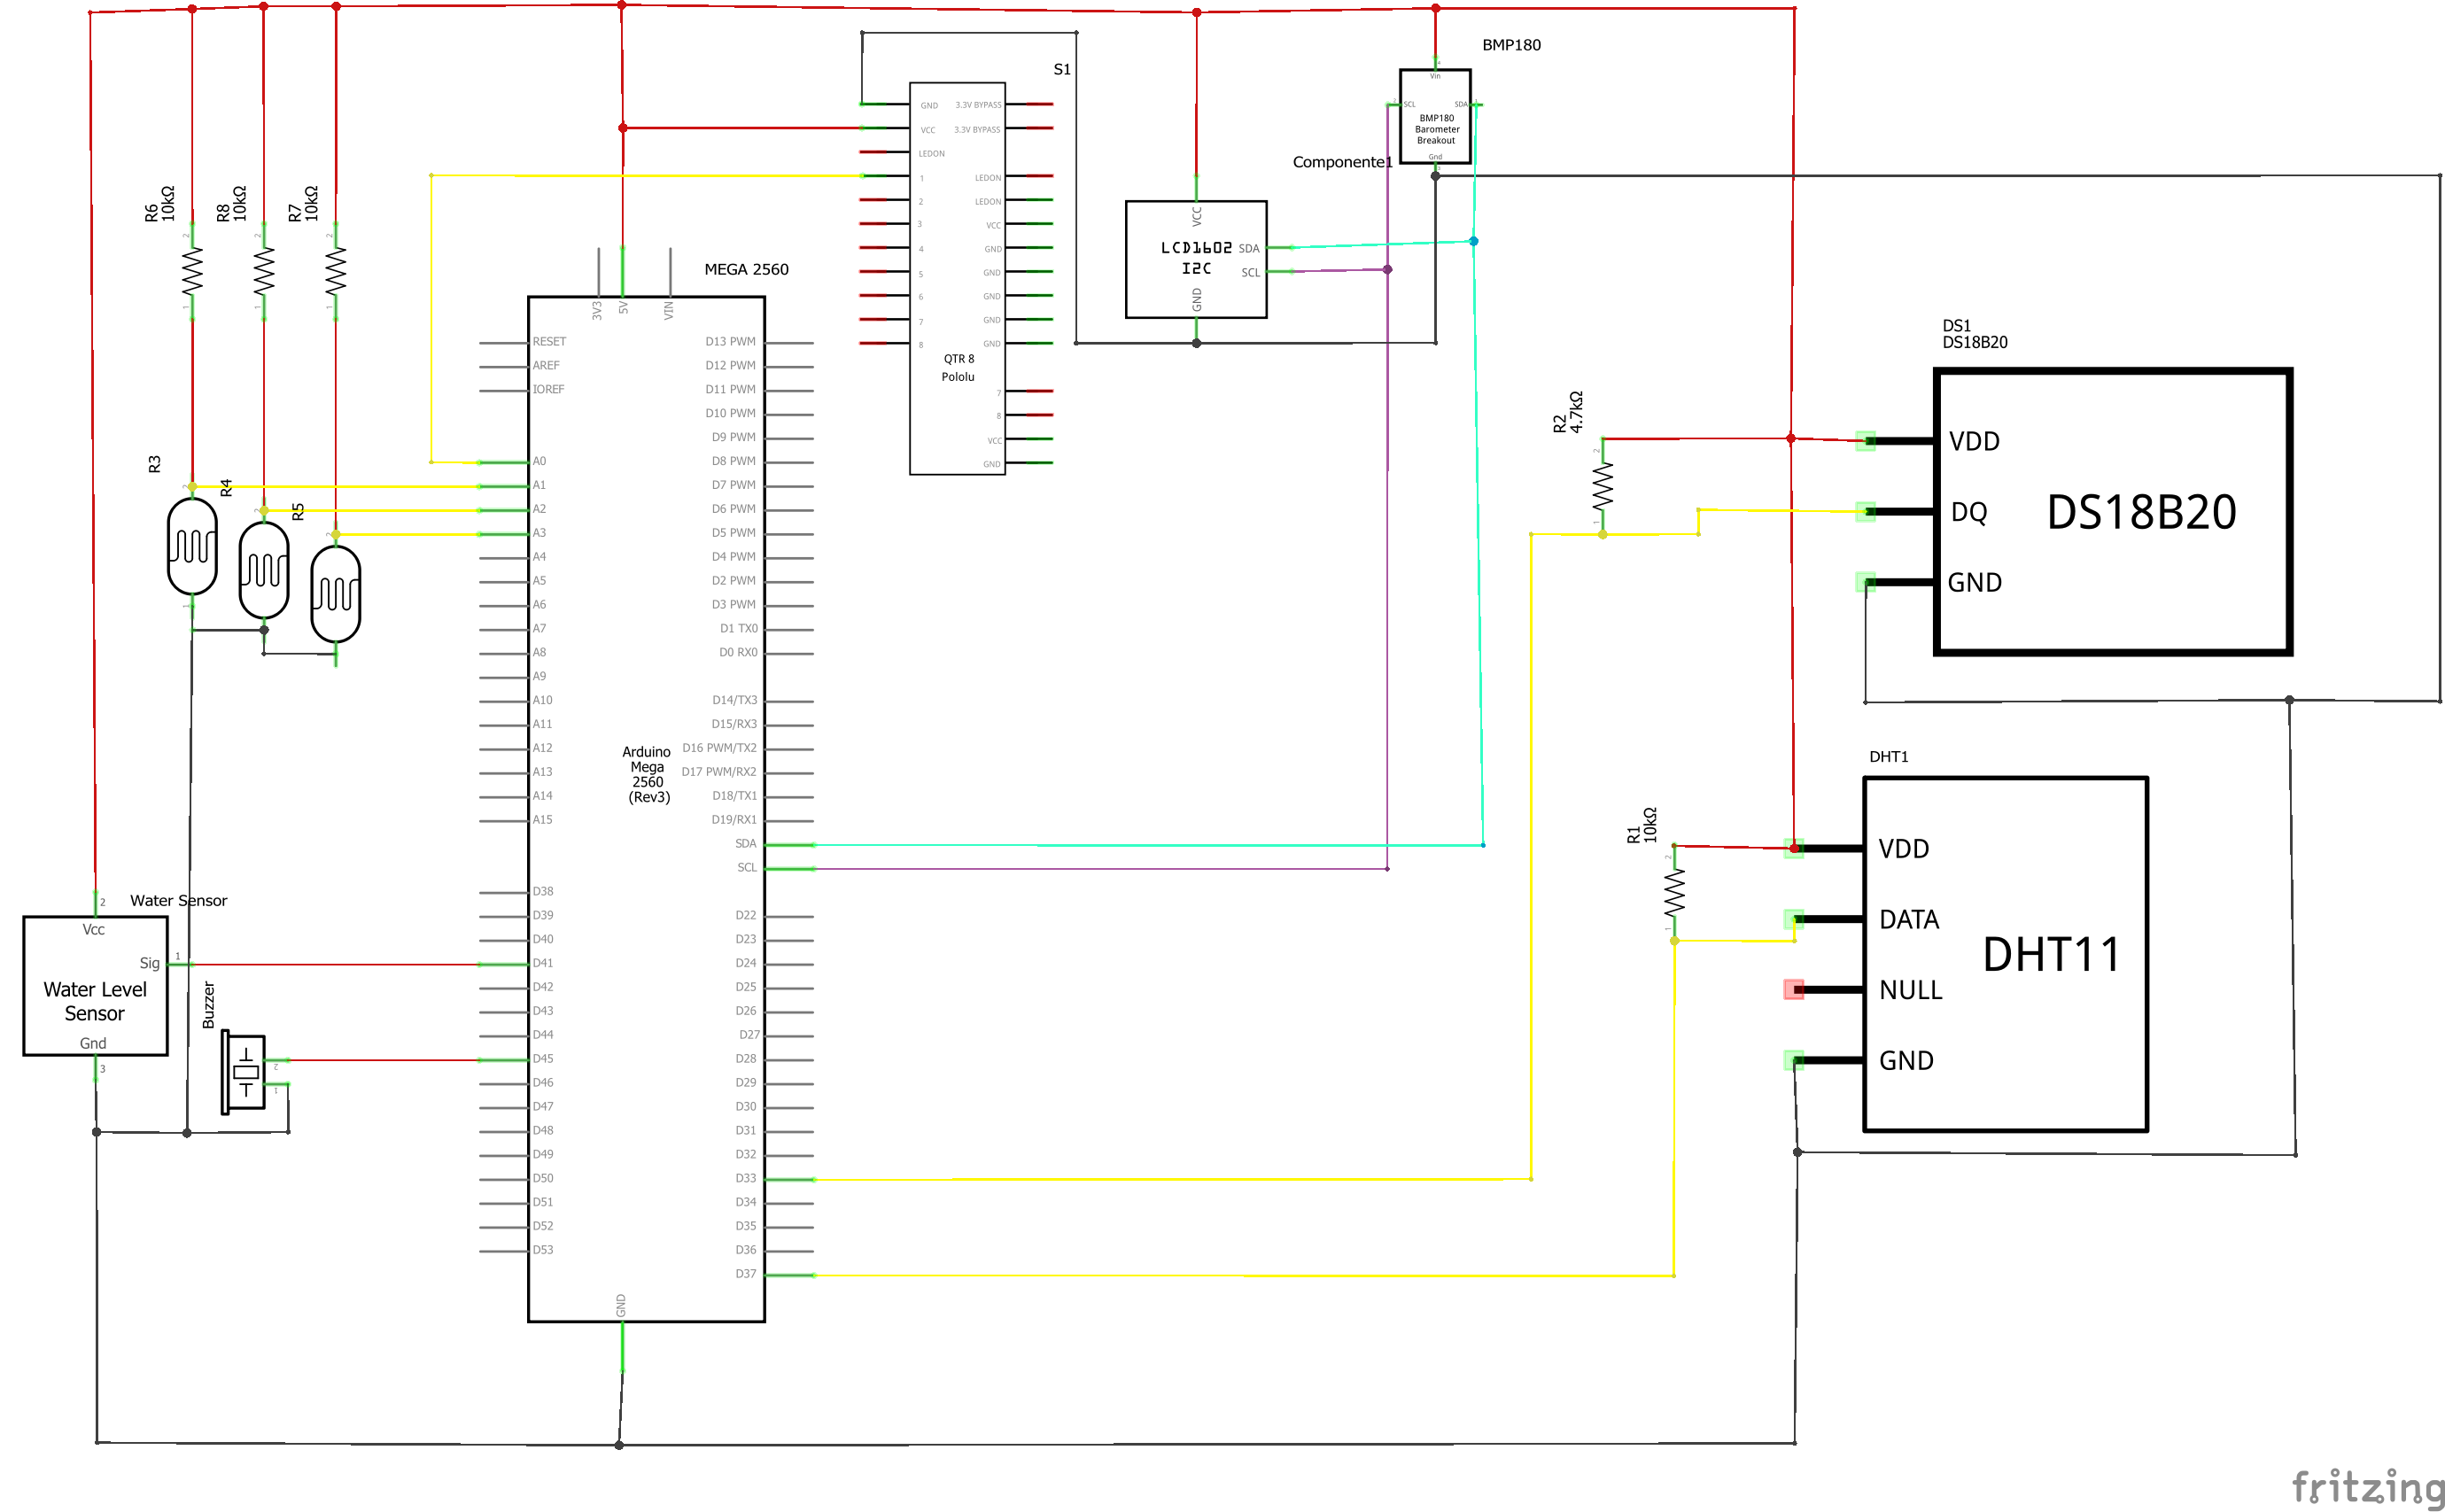
\includegraphics[width=\textwidth]{Prints/esquema.png}
\caption{Esquema do projeto}
\label{Rotulo}
\end{figure}

\newpage
Na imagem seguinte podemos ver o projeto finalizado.

\begin{figure} [!h]
\centering
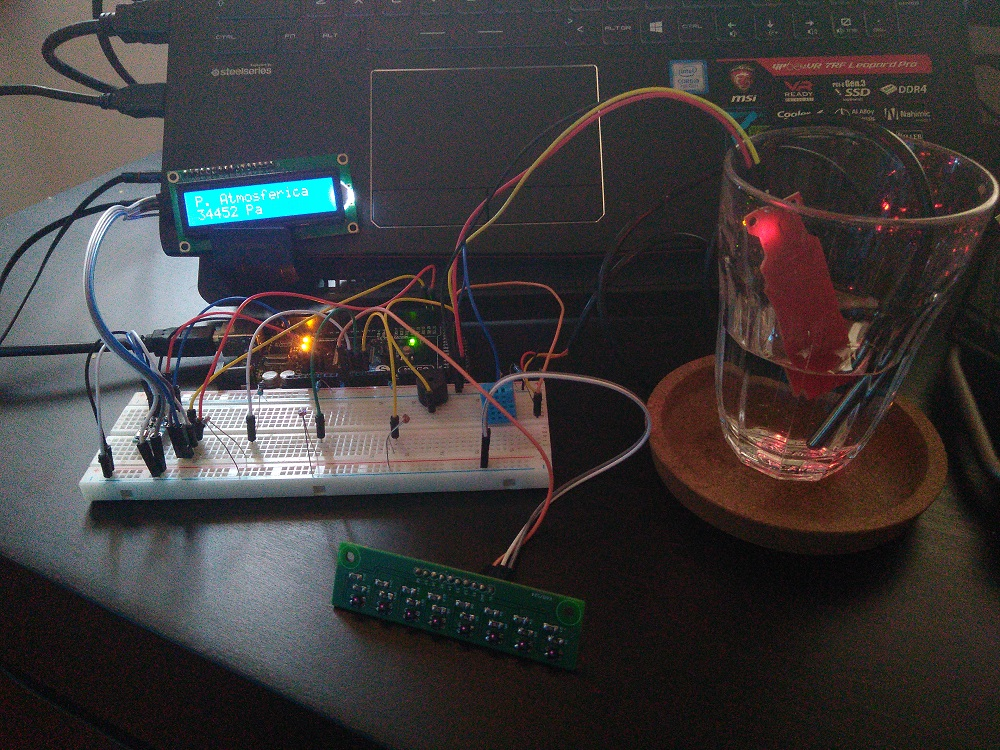
\includegraphics[width=\textwidth]{Prints/projecto.png}
\caption{Foto do projeto finalizado.}
\label{Rotulo}
\end{figure}



% Desenvolvimento
\chapter*{Desenvolvimento}
\addcontentsline{toc}{chapter}{Desenvolvimento}

Inicialmente decidimos que a nossa abordagem ao projeto seria começar por bare metal, testar todos os sensores e as ligações nesta metodologia de código e só depois passar à parte em que iríamos recorrer ao sistema operativo FreeRTOS. \linebreak

Começamos por testar o sensor de temperatura DS18B20 recorrendo à biblioteca OneWire.h \cite{OneWire}  para facilitar a leitura dos dados dos sensores. \cite{WaterproofDS18B20} \cite{sparkfunDS18B20}. De seguida, passamos ao sensor DHT11 que nos permite medir a percentagem de humidade do ambiente e a temperatura, para o qual adicionamos a biblioteca DHT.h \cite{DHTadafruit}. \cite{DHT}. Depois passamos ao barómetro BMP180, este sensor permite-nos medir a pressão atmosferica, a temperatura e com a pressão atmosferica podemos calcular aproximadamente a altitude que encontra.  Para obter os valores recorremos à biblioteca  Wire.h  (nativa do arduino) e a  Adafruit\_BMP085.h \cite{bmpBiblio}. \cite{bmp}. No final do circuito destes sensores montados e o código escrito, imprimimos o valor deste na consola para verificar se estava tudo a funcionar corretamente. \linebreak

O proximo passo foi testar o sensor de detecção de água, este foi bastante simples tendo em conta que devolve um sinal HIGH (5V) caso seja encontrada água nos contactos do sensor. \cite{water}. Depois montamos os 3 LDR's que servem para determinar a posição do sol, sendo estes também simples de instalar tendo em conta que já tínhamos experiência por termos feito circuitos com a utilização de LDR's no decorrer da cadeira. Só tivemos que os ligar e determinar no código qual dos LDR's estava a obter um valor de resistência mais baixo. \linebreak

Por fim, faltava utilização de LED's infravermelhos para ler a as rotações de um cata-vento, primeiro testamos utilizar simples LED's IR e contar as vezes que este era interrompido num certo período de tempo. Não obtendo sucesso recorremos ao sensor QTR-8RC mas utilizamos apenas um dos seus conjuntos de LED's. Para obter a leitura das Rotações por minuto fizemos uma função que durante 5 segundos consulta o valor obtido na porta analógica do LED receptor de 50 em 50 milissegundos. Caso este valor seja inferior ao do threshold definido (800) conta uma volta. Também tivemos que definir uma flag para evitar as mesmas leitura (caso o cata-vento estive-se parado). Para calcular um valor das rotações por minuto efetuamos uma regra de 3 simples para efetuar uma estimativa das rotações num minuto. \pagebreak

Como podemos verificar na imagem seguinte, estávamos a obter os valores dos sensores todos na consola.


\begin{figure} [!h]
\centering
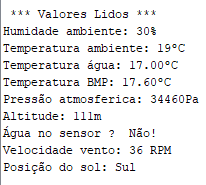
\includegraphics[width=50mm]{Prints/valores_consola.png}
\caption{Valores obtidos na consola do IDE.}
\label{Rotulo}
\end{figure}

O único aspecto que nos faltava para terminar a implementação em bare metal era mostrar os valores obtidos num LCD 16x2. Para facilitar a utilização do LCD recorremos a um modulo I2C que permite simplicar a ligação ao arduino usando as portas de comunicação SDA e SCL. Para utilizar o LCD recorremos a biblioteca LiquidCrystal\_I2C.h \cite{lcdbiblio}.  Podemos verificar na imagem seguinte o LCD a mostrar valores obtidos.


\begin{figure} [!h]
\centering
\includegraphics[width=100mm]{Prints/lcd.png}
\caption{LCD a mostrar o valor da altitude.}
\label{Rotulo}
\end{figure}

Ao desenvolver o código, até ao momento, tivemos o cuidado de poupar o máximo de memória possivel, até porque sabíamos que na implementação em FreeRTOS iríamos necessitar de toda a memória disponível. \cite{memoria}

O passo seguinte e final foi migrar o código desenvolvido até ao momento para utilizar o sistema operativo FreeRTOS. Para utilizar este tivemos que utilizar a biblioteca Arduino\_FreeRTOS.h \cite{rtos} e depois criamos 3 tarefas diferentes:

\begin{itemize}

\item \textit{GetSensorValuesTask} usada para obter os valores dos sensores.

\item \textit{ShowValuesLCDTask} usada para mostrar os valores obtidos no LCD.

\item \textit{PrintValuesOnConsoleTask} usada para mostrar os valores obtidos na consola do IDE.

\end{itemize}

Na imagem seguinte podemos verificar a criação das tarefas com os seus parâmetros únicos, tanto de tamanho, como de prioridade.

\begin{figure} [!h]
\centering
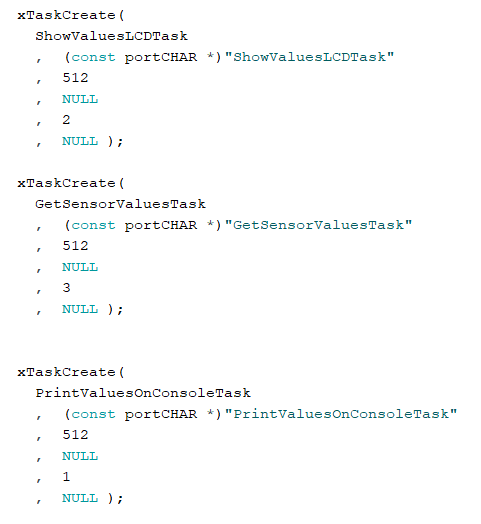
\includegraphics[width=55mm]{Prints/task.png}
\caption{Criação das tarefas.}
\label{Rotulo}
\end{figure}

\clearpage


Cada uma das tarefas reutiliza o mesmo código desenvolvido no bare metal, apenas às vezes com algumas alterações, como por exemplo, evitar a criação de variáveis dentro do ciclo infinito da tarefa para impedir ultrapassar o tamanho da stack e substituição dos delay's pelos  vTaskDelay's. Um dos problemas que nos surgiu nesta fase foi a escolha do tamanho da stack de cada tarefa. Para alcançarmos o tamanho ideal começamos por definir um valor alto para cada tarefa (ex: 1048 bits) e ir reduzindo até a tarefa deixar de funcionar. Chegamos ao valor mínimo de 512 bits para cada stack das tarefas.



\clearpage



% Conclução
\chapter*{Conclusão}
\addcontentsline{toc}{chapter}{Conclusão}

Este trabalho permitiu-se aplicar os conhecimentos adquiridos durante o decorrer da unidade curricular de Sistemas Embebidos e de Tempo Real. Achamos que o trabalho foi muito proveitoso porque tivemos pela primeira vez no curso um contacto com programação de mais baixo nível e onde trabalhássemos diretamente com o hardware. Foi muito interessante ter que ter cuidados com o tamanho das variáveis, tendo em conta que estávamos a trabalhar num ambiente onde a memória era muito escassa. De forma geral achamos que o trabalho correu suavemente, tendo em conta que ultrapassamos todas as dificuldades encontradas  e cumprimos todos os objetivos definidos pelo professor.

% Bilbiografia
\begin{thebibliography}{2}

	\bibitem{OneWire}
	 PaulStoffregen. \emph{OneWire.h}.  06 Abril, 2018. 
	\url{https://github.com/PaulStoffregen/OneWire}


	\bibitem{WaterproofDS18B20}
	dfrobot. \emph{Waterproof DS18B20 Digital Temperature Sensor}.  06 Abril, 2018. 
	\url{https://github.com/PaulStoffregen/OneWire}


	\bibitem{sparkfunDS18B20}
	sparkfun. \emph{DS18B20}.  06 Abril, 2018. 
	\url{https://github.com/sparkfun/simple_sketches/blob/master/DS18B20/DS18B20.ino}

	\bibitem{DHTadafruit}
	 Adafruit. \emph{Adafruit Unified Sensor Driver.}  06 Abril, 2018. 
	\url{https://github.com/adafruit/Adafruit_Sensor}

	\bibitem{DHT}
	 lady ada. \emph{Connecting to a DHTxx Sensor.}  06 Abril, 2018. 
	\url{https://learn.adafruit.com/dht/connecting-to-a-dhtxx-sensor}


	\bibitem{bmpBiblio}
	Adafruit. \emph{A powerful but easy to use BMP085/BMP180 Library.}  06 Abril, 2018. 
	\url{https://github.com/adafruit/Adafruit-BMP085-Library}


	\bibitem{bmp}
	 Adilson Thomsen. \emph{Controlando temperatura e pressão com o BMP180.}  06 Abril, 2018. 
	\url{https://www.filipeflop.com/blog/temperatura-pressao-bmp180-arduino/}


	\bibitem{water}
	 tutorialspoint. \emph{Arduino - Water Detector / Sensor.}  20 Abril, 2018. 
	\url{https://www.tutorialspoint.com/arduino/arduino_water_detector_sensor.htm}


	\bibitem{lcdbiblio}
	 fdebrabander. \emph{Library for the LiquidCrystal LCD display connected to an Arduino board.}  20 Abril, 2018. 
	\url{https://github.com/fdebrabander/Arduino-LiquidCrystal-I2C-library}


	\bibitem{memoria}
	 Bill Earl. \emph{Optimizing SRAM.}  30 Abril, 2018. 
	\url{https://learn.adafruit.com/memories-of-an-arduino/optimizing-sram}

	\bibitem{rtos}
	 feilipu. \emph{A FreeRTOS Library for all Arduino AVR Devices (Uno, Leonardo, Mega, etc) .}  06 Abril, 2018. 
	\url{https://github.com/feilipu/Arduino_FreeRTOS_Library}



\end{thebibliography}
\addcontentsline{toc}{chapter}{Bibliografia}

\end{document}